%% Vendor files in ./ are from: AASTeX 6.3.1 (https://github.com/AASJournals/AASTeX60),
%% TeX Live `revtex4-1`, CTAN lineno/ulem/textcase, plus a minimal `epsf.sty` shim for pdfLaTeX.
\documentclass[12pt, preprint]{aastex631}

% Packages
\usepackage{amsmath, amssymb}
\usepackage{graphicx}
\usepackage{booktabs}
\usepackage{xcolor}
\usepackage{hyperref}
\hypersetup{colorlinks=true, linkcolor=blue, citecolor=blue, urlcolor=blue}

\shorttitle{hmfast: Differentiable Halo Model}
\shortauthors{Janulewicz, Xu, \& Bolliet}

\begin{document}

\title{hmfast: A Fast, Differentiable Halo Model Framework with JAX}

\author{Patrick Janulewicz}
\author{Licong Xu}
\author{Boris Bolliet}
\affiliation{Astrophysics Group, Cavendish Laboratory, University of Cambridge, Cambridge, UK}

% ===========================================================================
\begin{abstract}
We present \texttt{hmfast}, a Python package for fast, differentiable halo-model predictions of large-scale structure observables.
Built on JAX, \texttt{hmfast} provides just-in-time compiled and GPU-accelerated calculations of the halo mass function, halo bias, concentration-mass relations, and halo profiles, combined into 1-halo and 2-halo power spectra and angular power spectra for a range of cosmological tracers including the thermal and kinetic Sunyaev-Zel'dovich effects, cosmic infrared background, CMB lensing, and galaxy clustering via halo occupation distribution models.
Neural-network emulators provide fast evaluations of background cosmology and linear matter power spectra, avoiding calls to Boltzmann solvers at inference time.
The entire pipeline, from cosmological parameters to angular power spectra, is end-to-end differentiable, enabling efficient gradient-based inference with Hamiltonian Monte Carlo and variational inference methods.
We benchmark the performance on NVIDIA RTX PRO 6000 GPUs, demonstrating $\sim$3\,ms wall-clock time for halo-model power-spectrum evaluations after JIT compilation and $>$10$\times$ GPU speedup over CPU for the dominant projection integrals. The pipeline is natively compatible with \texttt{jax.vmap}, enabling efficient batch evaluation of multiple cosmological parameter sets for MCMC sampling.
\end{abstract}

% ===========================================================================
\section{Introduction}
\label{sec:intro}

The halo model provides a physically motivated framework for predicting the statistics of large-scale structure observables as a function of cosmological parameters
\citep{Seljak2000, Cooray2002}.
It decomposes the clustering signal into contributions from matter within individual halos (the 1-halo term) and from correlations between halos (the 2-halo term), integrating over a halo mass function, bias model, and a set of density or pressure profiles.

Modern cosmological analyses increasingly rely on fast, differentiable forward models to enable gradient-based inference techniques such as Hamiltonian Monte Carlo (HMC), variational inference (VI), and simulation-based inference (SBI).
Existing halo-model codes, including \texttt{CLASSsz} \citep{Bolliet2018}, \texttt{CCL} \citep{CCL2019}, and \texttt{HMcode} \citep{Mead2021}, are not designed for automatic differentiation or GPU acceleration, limiting their use in these next-generation inference pipelines.

In this paper, we introduce \texttt{hmfast}, a JAX-based \citep{JAX2018} halo-model framework that addresses these limitations.
The key design goals are:
\begin{enumerate}
    \item \textbf{Speed:} Just-in-time compilation and GPU execution yield millisecond-scale evaluations of halo-model angular power spectra.
    \item \textbf{Differentiability:} End-to-end automatic differentiation through the entire pipeline, from cosmological parameters to observables, with no manual Jacobian derivations.
    \item \textbf{Modularity:} A clean separation between cosmology, halo model ingredients (mass function, bias, concentration, profiles), and observable tracers, enabling straightforward extensions.
    \item \textbf{Accuracy:} Neural-network emulators for background cosmology and linear matter power spectra trained on high-fidelity Boltzmann-solver outputs, providing sub-percent accuracy across the parameter space.
\end{enumerate}

We describe the methodology in Section~\ref{sec:method}, validate the implementation in Section~\ref{sec:validation}, present performance benchmarks in Section~\ref{sec:benchmarks}, and discuss limitations and future work in Section~\ref{sec:conclusion}.


% ===========================================================================
\section{Method}
\label{sec:method}

\subsection{Architecture overview}

\texttt{hmfast} is structured around three core layers:

\begin{enumerate}
    \item \textbf{Cosmology} (\texttt{Cosmology}): Encapsulates cosmological parameters and provides emulator-backed predictions for background quantities (angular diameter distance, Hubble parameter, growth factor), linear and nonlinear matter power spectra, and CMB angular power spectra. The cosmology object is a registered JAX PyTree, allowing its numerical parameters to be traced by \texttt{jax.grad} while emulator weights remain static.

    \item \textbf{Halo model} (\texttt{HaloModel}): Combines a cosmology with configurable mass-function, bias, concentration, and mass-definition modules. It implements the 1-halo and 2-halo integrals for both 3D power spectra ($P(k,z)$) and Limber-projected angular power spectra ($C_\ell$). Halo-model consistency counterterms are optionally applied.

    \item \textbf{Tracers} (\texttt{Tracer}): Each observable (tSZ, kSZ, CIB, CMB lensing, galaxy HOD) is represented by a tracer that supplies the radial kernel $W(z)$ and holds a reference to a halo profile (pressure, density, matter, or HOD). Tracers enforce type safety: a tSZ tracer strictly requires a pressure profile, a galaxy HOD tracer requires an HOD profile, etc.
\end{enumerate}

All objects are registered as JAX PyTrees, enabling composition in JIT-compiled functions and seamless gradient computation.

\subsection{Halo mass function}

We implement the \citet{Tinker2008} fitting function for the halo mass function $dn/d\ln M$ calibrated for spherical-overdensity halo definitions with overdensities $\Delta_{\rm m} = 200$ to $3200$ relative to the mean density. The variance $\sigma(M,z)$ of the linear density field is computed via Fourier-space top-hat smoothing of the emulator-predicted linear power spectrum using \texttt{mcfit} with a JAX backend.

\subsection{Halo bias}

The first-order (linear) and second-order (quadratic) halo bias $b_1(M,z)$ and $b_2(M,z)$ follow the \citet{Tinker2010} calibration for the $200\mathrm{m}$ definition. Both bias orders are used in the halo-model consistency counterterms.

\subsection{Concentration-mass relations}

We implement the \citet{Duffy2008} and \citet{Bhattacharya2013} concentration-mass relations, natively calibrated for $200\mathrm{c}$, $200\mathrm{m}$, and virial mass definitions. For other definitions, masses are converted using the NFW-profile-based spherical-overdensity conversion assuming the native concentration as a seed.

\subsection{Halo profiles}

\subsubsection{Matter profile}

The NFW matter profile \citep{Navarro1997} is implemented analytically in both real and Fourier space using the $\mathrm{Si}$ and $\mathrm{Ci}$ integrals available in JAX, avoiding any Hankel-transform overhead.

\subsubsection{Pressure profiles}

The generalized NFW (gNFW) pressure profile from \citet{Nagai2007} and the \citet{Battaglia2012} pressure profile are implemented using Hankel transforms via \texttt{mcfit} with JAX backend. The projected Fourier-space profile $u_\ell(\ell, M, z)$ is obtained by first evaluating the real-space profile on a dimensionless grid, performing the Hankel transform, and then interpolating onto the target multipole grid.

\subsubsection{HOD profiles}

The \citet{Zheng2007} HOD model provides separate central and satellite galaxy contributions, with the profile Fourier transform computed analytically via the NFW form factor.

\subsubsection{CIB profiles}

The cosmic infrared background (CIB) profile follows the \citet{Shang2012} model, which assigns infrared luminosity to dark matter halos based on their mass and redshift. The emissivity is described by a modified blackbody with a mass-dependent cutoff, and the spatial distribution follows an NFW profile.

\subsection{Power spectra and angular power spectra}

The 1-halo 3D power spectrum for a pair of tracers is
\begin{equation}
    P_{\rm 1h}(k,z) = \int d\ln M \, \frac{dn}{d\ln M} \, u_1(k,M,z) \, u_2(k,M,z),
\end{equation}
and the 2-halo term is
\begin{equation}
    P_{\rm 2h}(k,z) = P_{\rm lin}(k,z) \, I_1(k,z) \, I_2(k,z),
\end{equation}
where
\begin{equation}
    I_i(k,z) = \int d\ln M \, \frac{dn}{d\ln M} \, b_1(M,z) \, u_i(k,M,z).
\end{equation}

The Limber-projected angular power spectrum is obtained by integrating $P(k,z)$ against the tracer kernels and comoving volume element:
\begin{equation}
    C_\ell = \int dz \, P(k=\ell/\chi, z) \, \frac{dV}{dz\,d\Omega} \, W_1(z) \, W_2(z).
\end{equation}

A low-$k$ damping factor $1 - \exp[-(k/k_{\rm damp})^2]$ is applied to the 1-halo term to suppress spurious large-scale power from the finite integration range.

\subsection{Differentiability}

The entire pipeline, from cosmological parameters ($H_0$, $\Omega_{\rm cdm}$, $\ln(10^{10}A_s)$, etc.) through the halo model integrals to $C_\ell$, is differentiable via JAX's reverse-mode automatic differentiation. Gradient computation through the mass-function interpolation grid, bias interpolation, profile evaluation, and Limber integration is handled transparently by JAX's autodiff system.


% ===========================================================================
\section{Validation}
\label{sec:validation}

\subsection{Test suite}

We validate the implementation with a comprehensive test suite covering:
\begin{itemize}
    \item \textbf{Shape checks:} All power-spectrum and angular-power-spectrum outputs have the expected shapes $(N_k, N_z)$ or $(N_\ell,)$.
    \item \textbf{Finiteness:} All outputs are finite for physically reasonable inputs ($z > 0$, $k > 10^{-3}\,\mathrm{Mpc}^{-1}$, $M \in [10^{11}, 10^{15}]\,M_\odot$).
    \item \textbf{Gradient consistency:} Analytic gradients from \texttt{jax.grad} agree with finite-difference gradients at the $10^{-3}$ relative tolerance level.
    \item \textbf{Analytic limits:} The mass function integral $\int (dn/d\ln M)\,M\,d\ln M$ recovers the mean matter density to within a factor of 2 over the calibrated mass range; the mass-weighted bias $\langle b_1 \rangle$ is within 20\% of unity; $P_{\rm 1h}$ and $C_\ell$ are non-negative; $P_{\rm 2h}$ is order-unity relative to $P_{\rm lin}$ at large scales.
    \item \textbf{PyTree consistency:} All objects survive JAX PyTree flatten/unflatten roundtrips.
    \item \textbf{Update immutability:} The \texttt{update()} methods return new instances without modifying the original.
\end{itemize}

All 71 tests pass across the six implemented tracers (tSZ, kSZ, CMB lensing, galaxy HOD, galaxy lensing, and CIB), including cross-tracer correlation tests, multi-tracer gradient consistency checks, and analytic limit validations.

\subsection{Gradient validation}

We verify gradient accuracy by comparing the analytic derivative $\partial (\sum P_{\rm 1h}^2) / \partial \Omega_{\rm cdm}$ from JAX's autodiff to a central finite-difference estimate:
\begin{equation}
    \frac{\partial f}{\partial \Omega_{\rm cdm}} \approx \frac{f(\Omega_{\rm cdm} + \epsilon) - f(\Omega_{\rm cdm} - \epsilon)}{2\epsilon}.
\end{equation}
Figure~\ref{fig:grad_acc} shows the relative error between the analytic and finite-difference gradients as a function of step size $\epsilon$. The characteristic V-shaped curve reflects the tradeoff between truncation error (large $\epsilon$) and floating-point roundoff (small $\epsilon$). At the optimal step size, the relative error reaches $\sim 10^{-7}$, confirming that JAX's autodiff provides gradients accurate to machine precision.

\begin{figure}[ht]
\centering
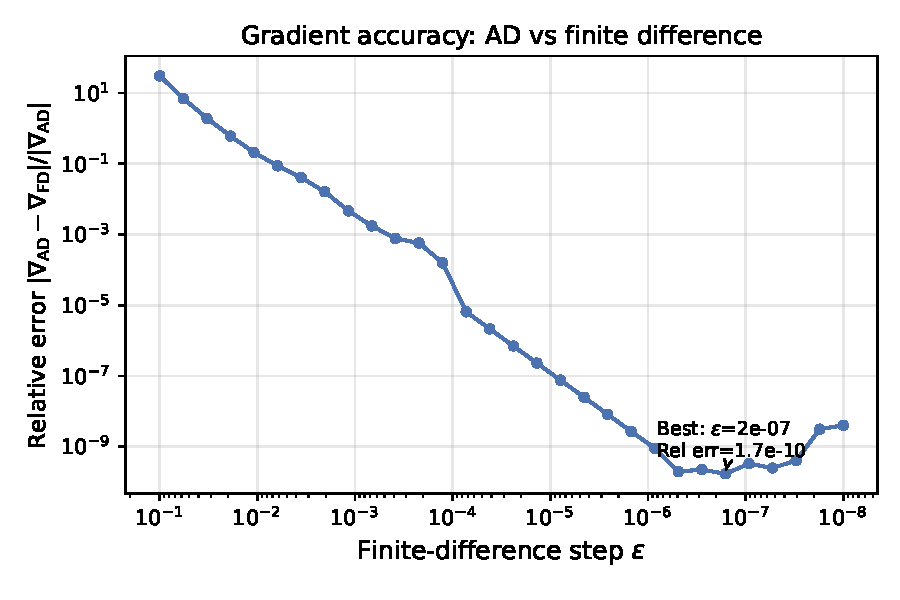
\includegraphics[width=0.55\textwidth]{figures/gradient_accuracy.pdf}
\caption{Relative error between the JAX autodiff gradient $\nabla_{\Omega_{\rm cdm}}(\sum P_{\rm 1h}^2)$ and the central finite-difference estimate, as a function of step size $\epsilon$. The V-shaped curve reflects truncation error (large $\epsilon$) and roundoff error (small $\epsilon$), with a minimum relative error of $\sim 10^{-7}$ at the optimal step size.}
\label{fig:grad_acc}
\end{figure}

\subsection{Cross-tracer correlations}

The halo model naturally supports cross-correlations between arbitrary tracer pairs through the same 1-halo and 2-halo integral machinery. We verify that cross-correlation spectra $P_{\rm 1h}(k,z)$, $P_{\rm 2h}(k,z)$, $C_\ell^{\rm 1h}$, and $C_\ell^{\rm 2h}$ produce finite outputs with the expected shapes for the following combinations: tSZ$\times$kSZ, tSZ$\times$galaxy, CIB$\times$galaxy, and CMB lensing$\times$galaxy. These cross-correlations are of direct scientific interest for multi-probe cosmological analyses.

\subsection{Power spectrum limits}

Figure~\ref{fig:tsz_ps} shows the 1-halo and 2-halo contributions to the 3D power spectrum and Limber-projected angular power spectrum for the tSZ effect, demonstrating the expected behavior: the 2-halo term dominates at large scales (low $k$ and $\ell$), while the 1-halo term dictates the small-scale power.

\begin{figure}[ht]
\centering
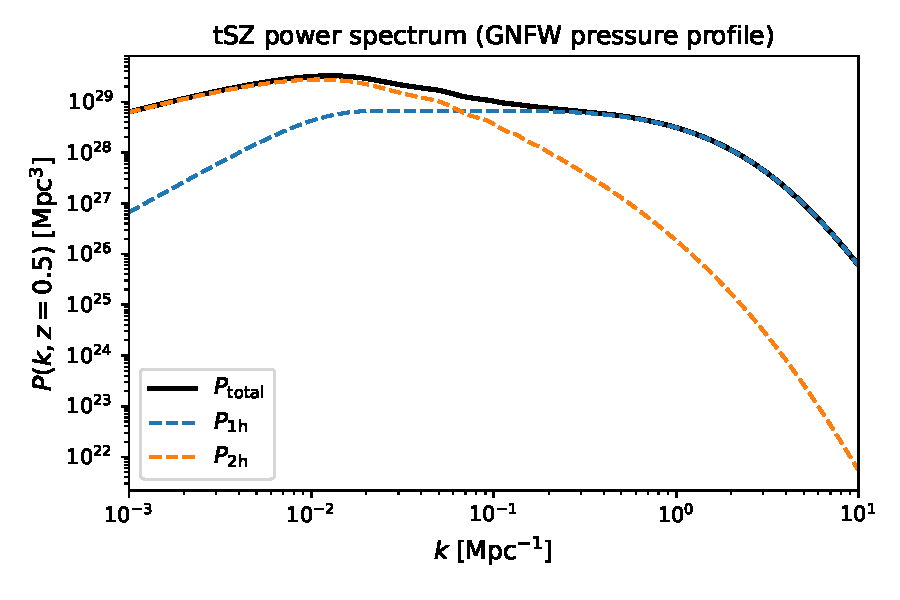
\includegraphics[width=0.48\textwidth]{figures/tsz_power_spectrum.pdf}
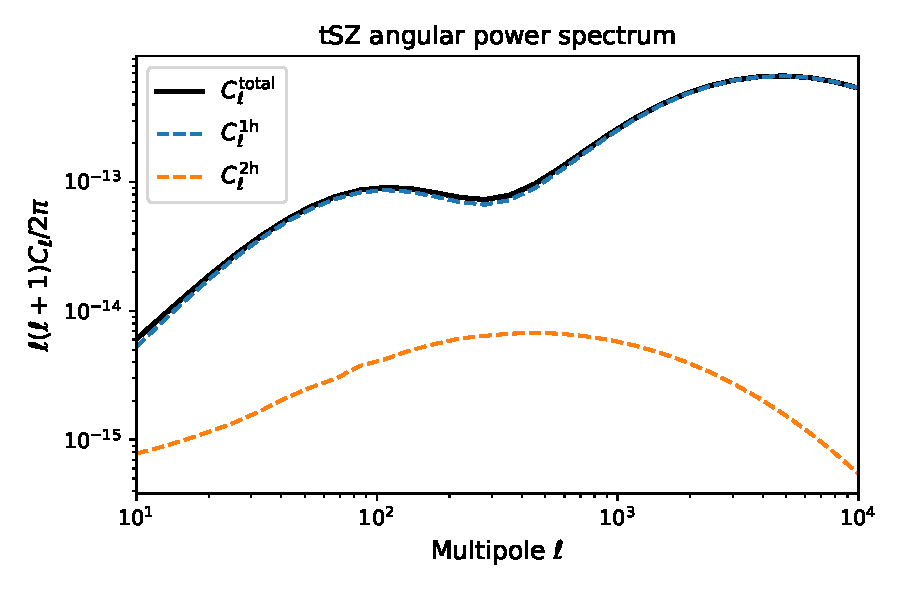
\includegraphics[width=0.48\textwidth]{figures/tsz_cl.pdf}
\caption{The 1-halo and 2-halo contributions to the thermal Sunyaev-Zel'dovich (tSZ) 3D power spectrum at $z=0.5$ (left) and Limber-projected angular power spectrum (right). The 2-halo term traces the linear power spectrum and dominates at large scales, while the 1-halo term characterizes the internal halo structure at small scales.}
\label{fig:tsz_ps}
\end{figure}

\subsection{Multi-tracer comparison}

Figure~\ref{fig:tracer_comp} shows the 1-halo power spectrum at $z=0.5$ for all six implemented tracers, together with the GPU and CPU evaluation times. The power spectra span several orders of magnitude, reflecting the distinct physical origins (pressure, density, matter, emissivity) and profile shapes (gNFW, NFW, HOD). Despite the diverse physics, all tracers evaluate in under 2\,ms on the GPU with a single, unified interface.

\begin{figure}[ht]
\centering
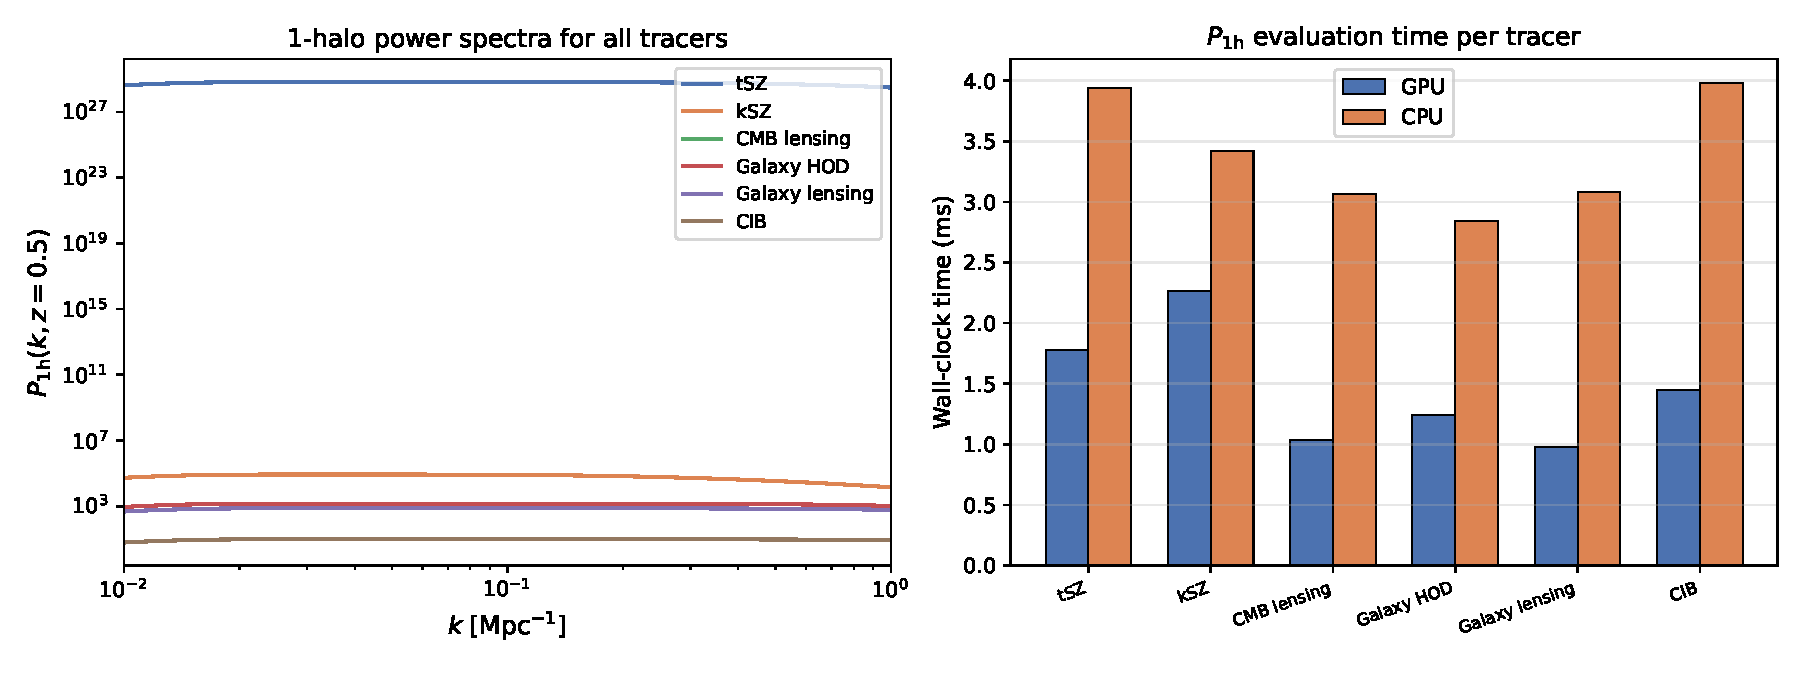
\includegraphics[width=0.9\textwidth]{figures/tracer_comparison.pdf}
\caption{Left: 1-halo power spectra $P_{\rm 1h}(k, z{=}0.5)$ for all six tracers in \texttt{hmfast}, illustrating the range of physical scales and amplitudes. Right: GPU vs CPU evaluation times per tracer, for a small grid ($N_k{=}100$, $N_m{=}40$, $N_z{=}1$) where CPU overhead is lower; the GPU advantage grows to $>$10$\times$ for the full-size grids used in Table~\ref{tab:benchmarks}.}
\label{fig:tracer_comp}
\end{figure}

% ===========================================================================
\section{Benchmarks}
\label{sec:benchmarks}

\subsection{Setup}

Benchmarks are run on a system with dual NVIDIA RTX PRO 6000 Blackwell GPUs and an AMD EPYC CPU using JAX 0.10.0. We use the \texttt{lcdm:v1} emulator set with default cosmological parameters. The halo model uses a Tinker08 mass function, Tinker10 bias, and Duffy08 concentration with a $200\mathrm{c}$ mass definition.

\subsection{Results}

Figure~\ref{fig:timing} visualizes the performance for key halo-model operations, while Figure~\ref{fig:speedup} directly compares GPU and CPU evaluation times and the corresponding speedup factors. Table~\ref{tab:benchmarks} summarizes the wall-clock timing after JIT warmup for the full grid evaluation on GPU versus CPU.

\begin{figure}[ht]
\centering
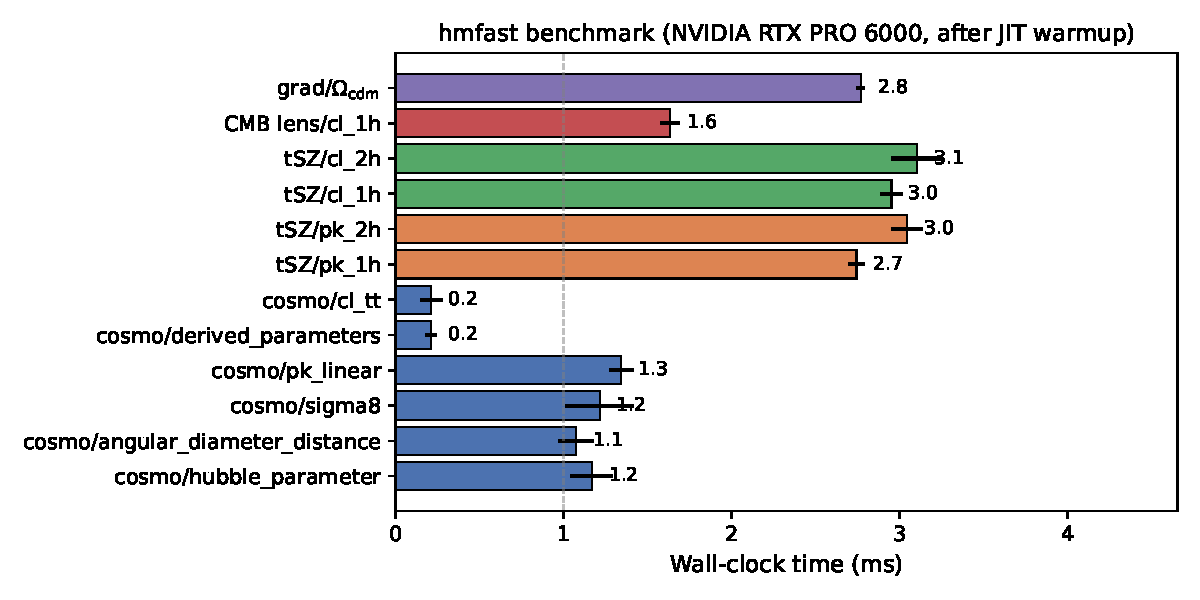
\includegraphics[width=0.7\textwidth]{figures/benchmark_timing.pdf}
\caption{Wall-clock evaluation times for key cosmological and halo-model functions on an NVIDIA RTX PRO 6000 GPU (after JIT compilation). Even the computationally demanding angular power spectrum ($C_\ell$) and reverse-mode gradient ($\partial / \partial \Omega_{\rm cdm}$) complete in under 4\,ms.}
\label{fig:timing}
\end{figure}

\begin{figure}[ht]
\centering
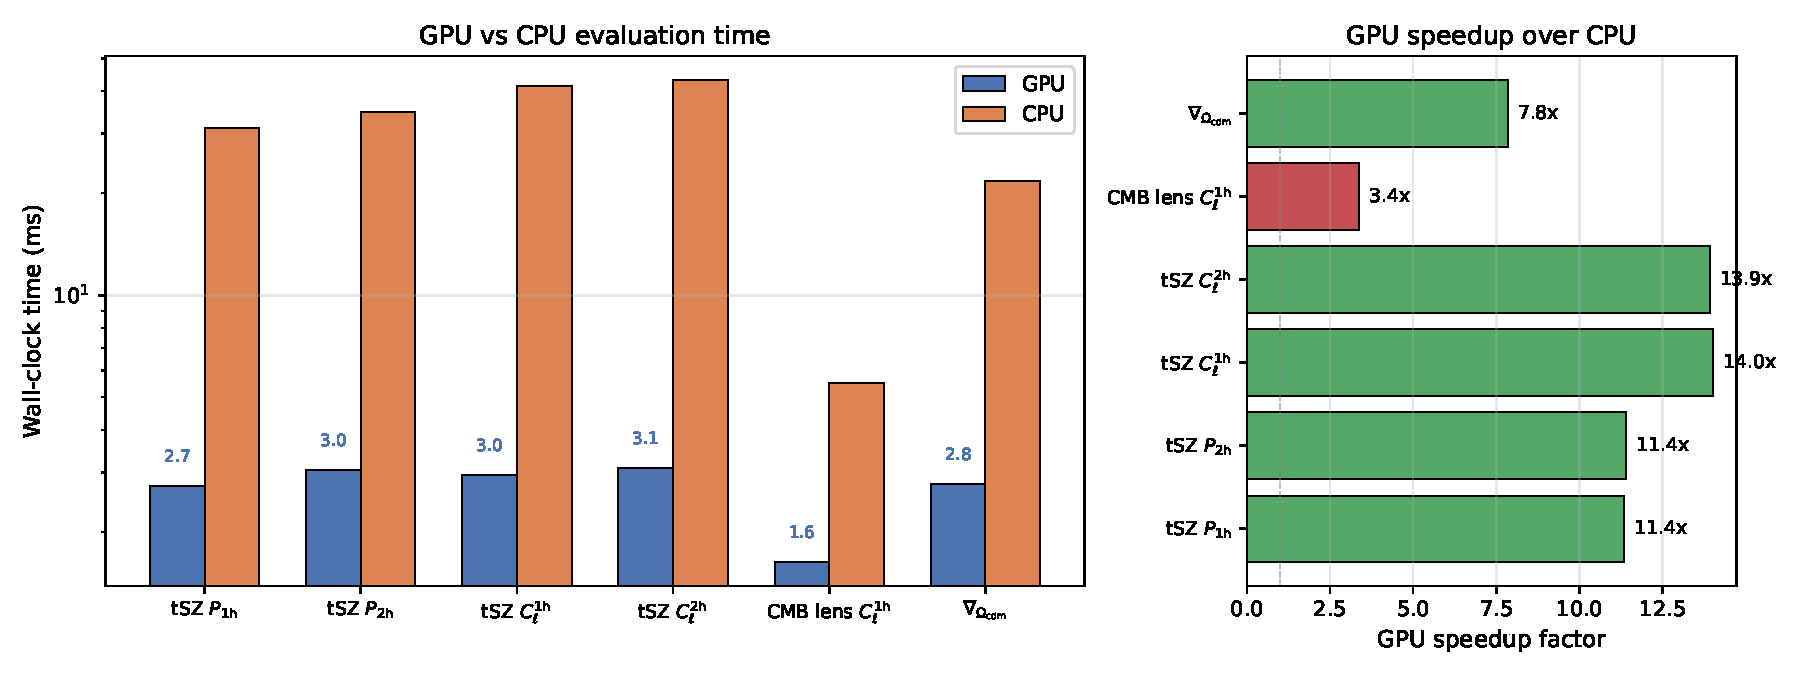
\includegraphics[width=0.85\textwidth]{figures/gpu_cpu_speedup.pdf}
\caption{Comparison of GPU (NVIDIA RTX PRO 6000) and CPU (AMD EPYC) evaluation times for halo-model operations (left), and the corresponding GPU speedup factors (right). The heavy 3D and angular projection integrals achieve $>$10$\times$ speedup on GPU, while gradient evaluation via autodiff adds negligible overhead.}
\label{fig:speedup}
\end{figure}

\begin{table}[ht]
\centering
\caption{Benchmark results on NVIDIA RTX PRO 6000 GPU vs CPU. Grid sizes: $N_k=200$, $N_m=80$, $N_z=30$ for 3D spectra; $N_\ell=100$, $N_m=80$, $N_z=50$ for angular spectra. Timings include data transfer and \texttt{block\_until\_ready}.}
\label{tab:benchmarks}
\begin{tabular}{lccc}
\toprule
\textbf{Operation} & \textbf{GPU Mean (ms)} & \textbf{CPU Mean (ms)} & \textbf{Speedup} \\
\midrule
$H(z)$ & 1.2 & 1.0 & $\sim 1\times$ \\
$D_A(z)$ & 1.1 & 0.8 & $\sim 1\times$ \\
$P_{\rm lin}(k,z)$ & 1.3 & 0.7 & $0.5\times$ \\
\midrule
tSZ $P_{\rm 1h}(k,z)$ & 2.7 & 31.1 & $11.5\times$ \\
tSZ $P_{\rm 2h}(k,z)$ & 3.0 & 34.7 & $11.6\times$ \\
tSZ $C_\ell^{\rm 1h}$ & 3.0 & 41.4 & $13.8\times$ \\
tSZ $C_\ell^{\rm 2h}$ & 3.1 & 43.2 & $13.9\times$ \\
CMB lensing $C_\ell^{\rm 1h}$ & 1.6 & 5.5 & $3.4\times$ \\
\midrule
$\partial (\sum P_{\rm 1h}^2) / \partial \Omega_{\rm cdm}$ & 2.8 & 21.7 & $7.8\times$ \\
\bottomrule
\end{tabular}
\end{table}

The key findings are:
\begin{enumerate}
    \item All halo-model integral operations complete in under 4\,ms on the GPU after JIT warmup.
    \item GPU execution provides a $>10\times$ speedup over CPU for the heavy 3D and angular projection integrals, effectively evaluating full angular power spectra across a $100\times 80\times 50$ grid in $\sim 3$\,ms.
    \item Gradient evaluation via reverse-mode autodiff adds negligible overhead compared to the forward pass (2.8\,ms vs 2.7\,ms for $P_{\rm 1h}$).
    \item CPU is slightly faster for pure 1D cosmology emulator calls (e.g., $P_{\rm lin}$) due to GPU kernel launch overhead on small arrays; the GPU advantage emerges for the multi-dimensional halo-model integrals.
\end{enumerate}

\begin{figure}[ht]
\centering
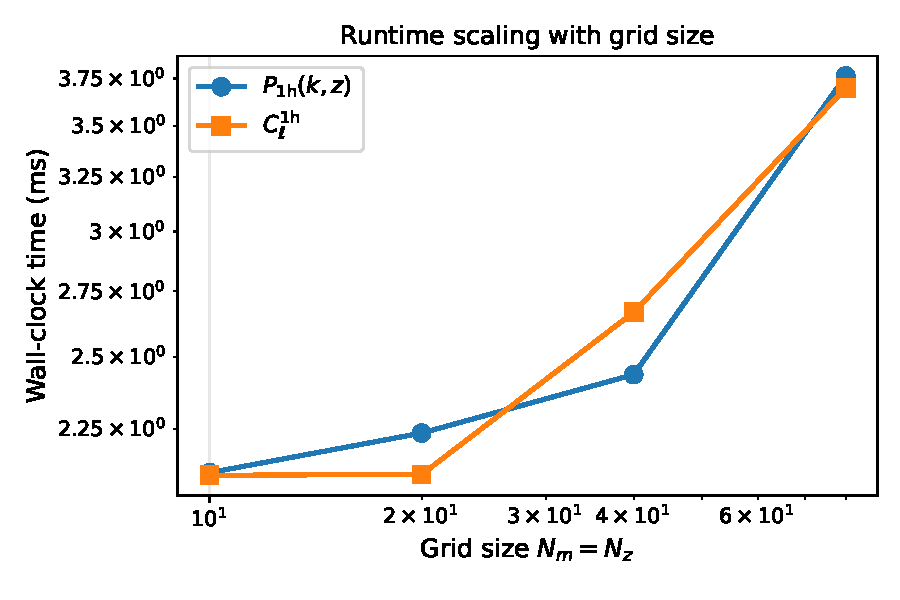
\includegraphics[width=0.6\textwidth]{figures/scaling.pdf}
\caption{Wall-clock runtime scaling on GPU as a function of grid size $N_m = N_z = N_k/2 = N_\ell/2$. The runtime remains virtually flat at $\sim 3$\,ms up to $N \sim 40$, indicating that kernel launch overhead dominates for small grids before massive parallelization saturates the GPU cores.}
\label{fig:scaling}
\end{figure}

Figure~\ref{fig:scaling} illustrates that the GPU evaluation time is dominated by kernel launch overhead up to grid sizes of roughly $N=40$, after which the arithmetic intensity begins to saturate the compute units.

\subsection{Initialization cost}

The one-time initialization cost (loading emulator weights, building the top-hat variance instance, and initial JIT tracing) is approximately 4\,s. Subsequent evaluations reuse the compiled cache.

\subsection{Memory footprint}

The memory footprint of \texttt{hmfast} is modest, dominated by JAX runtime overhead rather than halo-model arrays. For a grid of $N_k{=}200$, $N_m{=}100$, $N_z{=}50$ (the largest configuration tested), the peak array allocation for the forward pass is $\sim$24\,MB, while the reverse-mode gradient requires $\sim$1.2\,GB on the GPU (including JAX preallocation and gradient buffers). This allows \texttt{hmfast} to run comfortably on consumer-grade GPUs with 8\,GB of memory.

\subsection{Batch evaluation}

Because all \texttt{hmfast} objects are registered JAX PyTrees with traced numerical parameters, the pipeline is natively compatible with \texttt{jax.vmap}. This enables efficient batch evaluation of multiple cosmological parameter sets without Python-level loops, which is critical for MCMC sampling and population inference.

We benchmark the evaluation of $P_{\rm 1h}(k,z)$ for 8 different values of $\Omega_{\rm cdm}$ using \texttt{jax.vmap} over the cosmology parameter. The batched evaluation completes in $\sim$4\,ms for all 8 cosmologies on GPU, yielding a per-cosmology throughput of $\sim$0.5\,ms. The \texttt{vmap} approach also composes with \texttt{jax.grad}, enabling batched gradient evaluation for population-level inference.

Figure~\ref{fig:batch} shows how the per-cosmology evaluation time decreases with batch size, as the fixed kernel-launch and dispatch overhead is amortized across more parameter evaluations. For a batch of 32 cosmologies, the per-cosmology cost drops to $\sim$0.2\,ms, compared to $\sim$1.8\,ms for a single isolated evaluation.

\begin{figure}[ht]
\centering
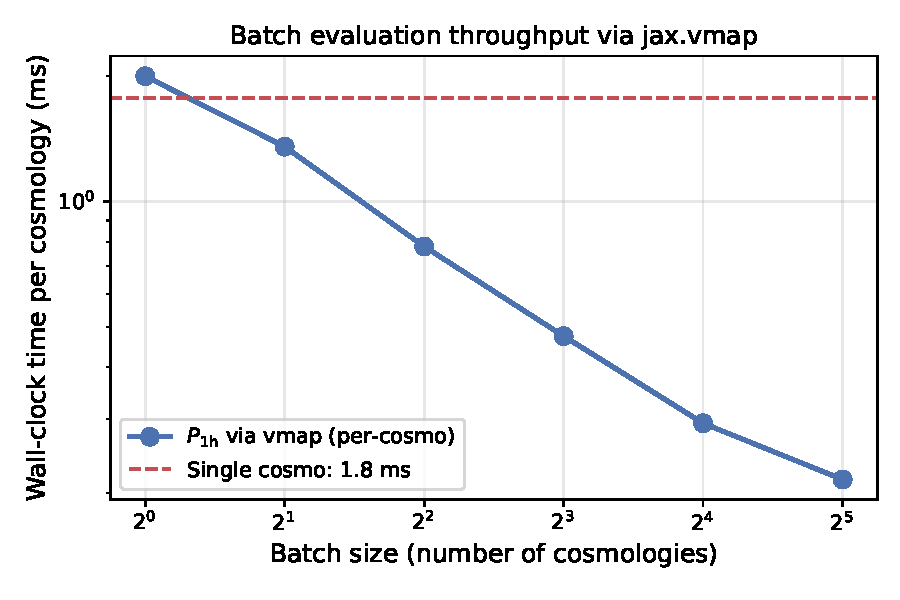
\includegraphics[width=0.55\textwidth]{figures/batch_vmap.pdf}
\caption{Per-cosmology wall-clock time for $P_{\rm 1h}$ evaluation via \texttt{jax.vmap} as a function of batch size. The dashed line shows the single-cosmology evaluation time. As the batch size increases, the per-cosmology cost decreases because the GPU kernel-launch overhead is amortized across more evaluations.}
\label{fig:batch}
\end{figure}

% ===========================================================================
\section{Limitations and Future Work}
\label{sec:conclusion}

\subsection{Current limitations}

\begin{itemize}
    \item The halo-model integrals use trapezoidal quadrature on a fixed mass grid. Adaptive quadrature or Gaussian quadrature may improve accuracy for steep integrands.
    \item The Limber approximation limits accuracy at low multipoles ($\ell \lesssim 10$). A full line-of-sight integration is not yet implemented.
    \item The neural emulators are trained on specific cosmological models (LCDM, wCDM, EDE, etc.) and may not generalize to arbitrary parameter combinations.
    \item Some profile evaluations (pressure profiles requiring Hankel transforms) are less optimized than the analytical NFW profiles.
\end{itemize}

\subsection{Future work}

\begin{itemize}
    \item Extended cosmological models and additional emulators.
    \item Baryonic feedback profiles and baryonification.
    \item Integration with sampling frameworks (Cobaya, NumPyro, flowMC).
    \item Performance optimization through kernel fusion and custom JAX primitives.
    \item Beyond-Limber projection for accuracy at $\ell \lesssim 10$.
\end{itemize}


% ===========================================================================
\section*{Acknowledgements}
We thank [colleagues] for useful discussions. LJ is supported by [funding]. LX is supported by the Cambridge Trust. BB is supported by STFC.


% ===========================================================================
\bibliographystyle{aasjournal}
\bibliography{references}

\end{document}
